\chapter{Implementation}

In this chapter we describe implementation details in developed software and describe it's functionality on examples. We will use following example to show optimizations and compiling:


\begin{verbatim}
select
    l_orderkey,
    sum(l_extendedprice*(1-l_discount)) as revenue,
    o_orderdate,
    o_shippriority
from
    customer,
    orders,
    lineitem
where
    c_mktsegment = '[SEGMENT]'
    and c_custkey = o_custkey
    and l_orderkey = o_orderkey
    and o_orderdate < date '[DATE]'
    and l_shipdate > date '[DATE]'
group by
    l_orderkey,
    o_orderdate,
    o_shippriority
order by
    revenue desc,
    o_orderdate;
\end{verbatim}

This example is taken from Tpc benchmark \cite{benchmark}. $[DATE]$ and $[SEGMENT]$ are constants. In this benchmark there are no indexes on tables. Columns which starts wit o\_ are from table order, columns which beginning with l\- are from table lineitem and columns starting with \_c belongs table customers.



\section{Input}

As mentioned input is XML containing logical query plan. In this section we describe it's structure. 

\subsection{Sort}

On root of every tree is sort, even if output hasn't been sorted. in this case it has empty parameters. This is an example of sort in algebra tree:


\lstset{
  language=XML,
  morekeywords={encoding,
    xs:schema,xs:element,xs:complexType,xs:sequence,xs:attribute}
}
\begin{lstlisting}
<?xml version="1.0" encoding="utf-8"?>
<sort xmlns:xsi="http://www.w3.org/2001/XMLSchema-instance"
 xsi:noNamespaceSchemaLocation="algebra.xsd">
  <parameters>
    <parameter column="revenue" direction="desc" />
    <parameter column="o_orderdate" direction="asc" />
  </parameters>
  <input>
  ...
  <input>
</sort>
\end{lstlisting}

Sort is a root element of XML file. Inside parameters is specified how to sort relation. In this example we have sort $\tau_{revenue:desc,o\_orderdate:asc}(...)$. In element input there should be one other algebra tree node.

\subsection{Group}

Next example display group node:

\begin{lstlisting}
<group>
  <parameters>
    <group_by column="l_orderkey"/>
    <group_by column="o_orderdate" />
    <group_by column="o_shippriority"/>
    <sum argument="x" output="revenue"/>
  </parameters>
  <input>
  ...
  <input>
</group>
\end{lstlisting}

This node represents expression $\gamma_{l\_orderkey,o\_orderdate,o\_shippriority,x=sum(x)}(...)$. Group element has to have at least one group by parameter or at least one aggregate function. Inside element input there should be one other operator.

\subsection{Selection}

This is an example of selection:

\begin{lstlisting}

<selection>
  <parameters>
    <condition>
      <lower>
        <constant type="date" value="today"/>
        <column name="l_shipdate"/>
      </lower>
    </condition>
  </parameters>
  <input>
  ...
  </input>
</selection>
\end{lstlisting}
This example represent following expression: $\sigma_{today<l_shipdate}$. In condition element we can have multiple conditions connected by $and$ or $or$ elements. Input algebra supports operators $=$,$<$ and $\leq$. In the leafs of expression tree there can be only column or constant element. We also can call a boolean function from condition, which is represented in following example.

\begin{lstlisting}
<condition>
  <boolean_predicate  name="like">
    <argument>
      <column name="x"/>
    </argument>
    <argument>
      <constant type="int" value="445" />
    </argument>
  </boolean_predicate>
</condition>
\end{lstlisting}

While using boolean predicate it has to be supported by runtime(Bobox operators). Compile doesn't check it's existence.

\subsection{Join}

Join without condition is considered to be cross join. We can use join with multiple equal conditions or with simple unequal condition. First example contains equal conditions:

\begin{lstlisting}
<join>
  <parameters>
    <equal_condition>
      <equals>
        <column name="a"/>
        <column name="b"/>
      </equals>
      <equals>
        <column name="c"/>
        <column name="d"/>
      </equals>
    </equal_condition>
    <column name="a" input="first"/>
    <column name="b" input="second"/>
    <column name="c" input="first"/>
    <column name="d" input="second" newName="e" />
  </parameters>
<input>
...
</input>
\end{lstlisting}

This example represents join with condition $a=b~and~c=d$. In join equal conditions has to be first column from first relation and second column from second relation. In example $a$ and $c$ are from first input and $b$ and $d$ are from the other one. Joins doesn't copy to output all column from both input relations. After condition we have to specify non empty sequence of columns. In every column we specify it's name and number of input. We can also rename join output column by using attribute $newName$. In example we renamed column $d$ to $e$.

Next example shows also join but with inequality condition:

\begin{lstlisting}
<join>
  <parameters>
    <less_condition>
      <and>
        <lower_or_equals>
          <column name="a1"/>
          <column name="b"/>
        </lower_or_equals>
      <lower_or_equals>
        <column name="b"/>
        <column name="a2"/>
      </lower_or_equals>
    </and>
  </less_condition>
  <column name="a1" input="first"/>
  <column name="b" input="second"/>
  <column name="a2" input="first"/>
</parameters>
<input>
...
</input>
</join>
\end{lstlisting}
This example represents join with condition $a1\leq b\leq a2$. In first sub condition first column has to be from first input, but in second sub condition first column has to be from second input. Also instead $lower\_or\_equals$ we can use just $lower$ condition. Rules for output column are same like in join with equal conditions.

In element $input$ of join there has to be two operators.

\subsection{Anti join}

\begin{lstlisting}
<antijoin>
  <parameters>
    <equal_condition>
      <equals>
        <column name="d"/>
        <column name="b"/>
      </equals>
    </equal_condition>
    <column name="d"/>
  </parameters>
<input>
...
<input>
</antijoin>
\end{lstlisting}
This is an example of antijoin with simple condition $d=b$. Structure is the almost same like join. Output columns can be only from first relation and we can also rename this columns.

\subsection{Table}
This is a leafs of algebra tree. It specifies name of read table, its columns and indexes. We can specify number of rows in the table to get better plans. If it is not specified we will assume that table has 1000 tuples. For every column we have to specify name and it's type. Other optional parameter is $number\_of\_unique\_values$. This number is important for estimating size of join. If it is not given, we will assume, that $number\_of\_unique\_values$ is size of table to power of $\frac{4}{5}$. This assumption is only experimental, since number of unique values can be from $0$ to size of table. Index can be clustered or unclustered. Table can have only one clustered index. In every index we specify on what attribute it is created. Here is an example or table algebra node:
 
\begin{lstlisting}
<table name="orders" numberOfRows="1500000">
  <column name="o_orderdate" type="int"/>
  <column name="o_shippriority" 
  type="int" number_of_unique_values="30000"/>
  <column name="o_orderkey" type="int"/>
  <column name="o_custkey" type="int" />
  <index type="clustered" name="index">
    <column name="o_orderdate" order="asc" />
    <column name="o_shippriority" order="asc" />
  </index>
</table>
\end{lstlisting}

\subsection{Union}
Union doesn't have any parameters, but columns from both input have tt have the same name. Here is an example:
\begin{lstlisting}
<union>
  <input>
  ...
  </input>
</union>
\end{lstlisting}

\subsection{Extended projection}
Following example of extended projection represents expression \\ $\pi_{l\_orderkey,o\_orderdate,o\_shippriority,x=l\_extendedprice*(1-l\_discount)}(...)$.
\begin{lstlisting}
<column_operations>
  <parameters>
    <column name="l_orderkey"></column>
    <column name="o_orderdate"></column>
    <column name="o_shippriority"></column>
    <column name="x">
      <equals>
        <times>
          <column name="l_extendedprice"/>
          <minus>
            <constant type="double" value="1"/>
            <column name="l_discount"/>
          </minus>
        </times>
      </equals>
    </column>
  </parameters>
  <input>
  ...
  </input>
</column_operations>
\end{lstlisting}

Extended projection contains list of columns. If columns is new computed values it contains elements representing expression tree. It cal also contain function call, which has to be supported by Bobox operators. Following example displays function call:


\begin{lstlisting}
<column_operations>
  <parameters>
    <column>
      <equals>
        <aritmetic_function name ="sqrt">
          <argument>
            <constant type="double" value="2"/>
          </argument>
        </aritmetic_function>
      </equals>
    </column>
  </parameters>
  <input>
    ...
  </input>
</column_operations>
\end{lstlisting}
 
\section{Building relational algebra tree} 

In this section we describe in more details structure storing logical plan and it's building.

Relational algebra operators are represented by children of abstract class \texttt{AlgebraNodeBase}. It has following abstract subclasses:
\begin{itemize}

\item \texttt{UnaryAlgebraNodeBase} - abstract class for algebra operator with one input

\item \texttt{BinaryAlgebraNodeBase}  - abstract class for algebra operator with two inputs

\item \texttt{GroupedAlgebraNode} - abstract class for algebra operator with variable number inputs

\item \texttt{NullaryAlgebraNodeBase} -  abstract class for algebra tree leafs

\end{itemize}

All operators are children of one of mentioned classes. Every operator has pointer to it's parent in tree and smart pointers to it's children if it has any. 

Expressions in nodes are represented by polymorphic trees. All expression nodes are children of class \texttt{Expression}.

For manipulating and reading expression and algebra tree we used visitor pattern. All nodes (algebra and expression) contains method \texttt{accept}. This method calls visitor method on class \texttt{AlgebraVisitor}/\texttt{ExpressionVisitor}. All classes, which manipulate algebra tree, are children of class \texttt{AlgebraVisitor}.


\begin{figure}[h!]
  \centering
    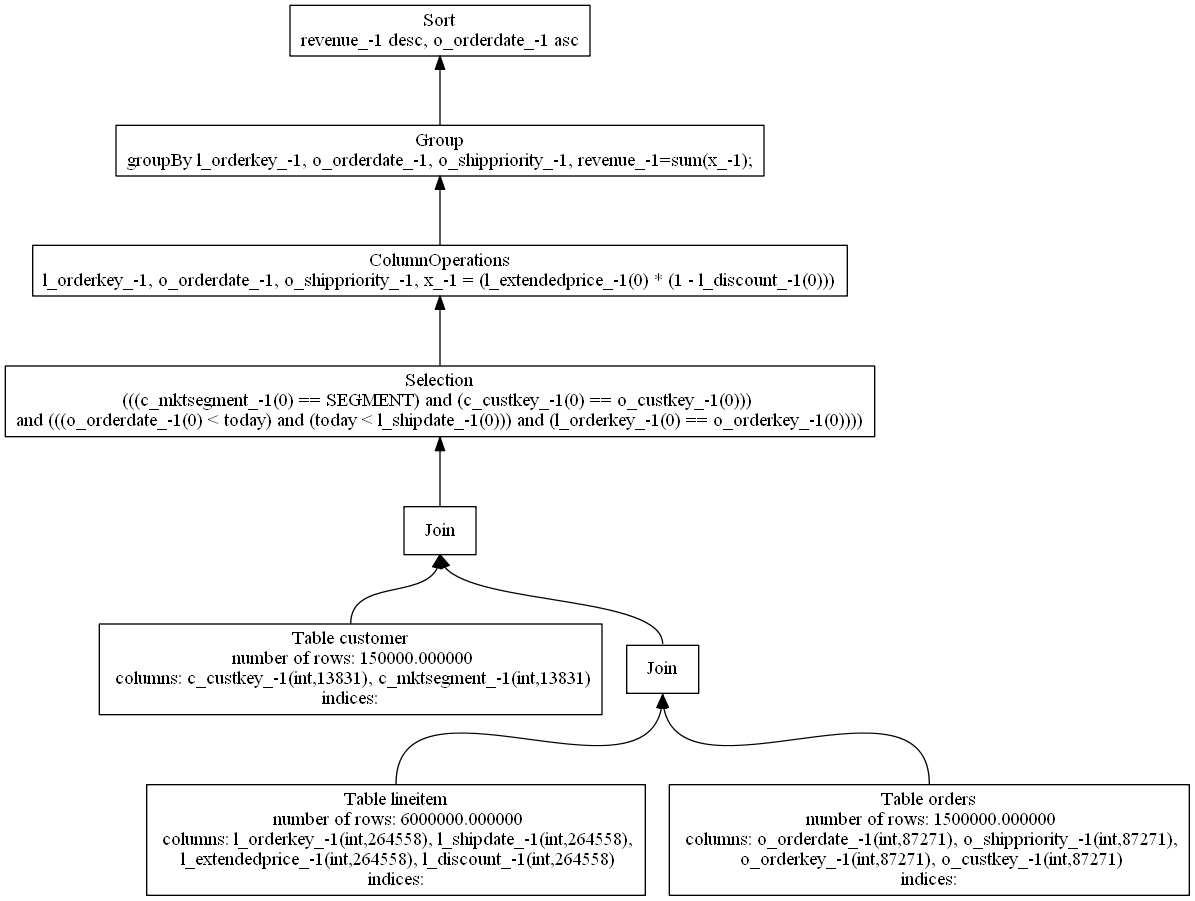
\includegraphics[width=1.0\textwidth]{algebratree1}

      \caption{Example of algebra tree.}
          \label{fig:algebratree1}
\end{figure}

In figure~\ref{fig:algebratree1} we have example of algebra tree of query presented in beginning in this chapter. We translated it as cross join of tree tables. After that we apply selection with condition in where clause. From the result we compute new column, group and sort result. In table reading operator we can see that they store additional information, like name of table. Every attribute has $\_-1$, behind name. It is it's unique identifier but after building tree from XML it is not assigned yet and that's why it contains default value $-1$. Columns in expressions also contains number in parenthesis. This number stores information from which input this columns it. Inputs are numbered from $0$. Here we can see that all columns in selection are from $0^{th}$ input. This information is useful mainly in joins.

For parsing and validating input XML file we used library Xerces version 3.1.1\cite{xerces}. It parses input file and create DOM tree. This tree has to be validated so we know it contains valid relational algebra tree. All this functionality is in class \texttt{XmlHandler}.

We know that every tree has to have sort operator on the top. We call \texttt{Sort} constructor on it. This method takes all information from DOM tree and call method, which decide that constructor to call next on it's children. This way we recursively build algebra tree.



\section{Semantic analysis and node grouping}

This phase in done in class \texttt{SemanticChecker}. It checks columns used in expression exist. It also checks if output columns of operator has unique name. During this checking we assign unique identifier to every column. After this phase we don't need names only this id.

Logical plan is after that visited by \texttt{GroupingVisitor}. In this phase are replaced joins represented by class \texttt{Join} by grouped join with two or more input relations. This node is represented by class \texttt{GroupedJoin}. Also in every expression we apply \texttt{GroupingExpressionVisitor}. It groups expression with $and$ and $or$ operators. This is done for simplifying splitting condition into sub conditions.

\section{Algebra optimization}

We need to prepare logical tree for optimizing it by pushing down selections. To do this we split selection into smaller conditions using rule:
\begin{itemize}
\item $\sigma_{A~and~B}(R)=\sigma_{A}(\sigma_{B}(R))$
\end{itemize}
From every selection we created chain of selections. This operation is done by \texttt{SelectionSpitingVisitor}.

After that we call \texttt{SelectionColectingVisitor}. This visitor stores pointer of all selection in relational algebra tree. This pointers are input into \texttt{Push\-Selection\-Down\-Visitor}. It pushes all selections down the tree as much as possible and also converts cross joins into regular joins if we have selection with equal condition.
\begin{figure}[h!]
  \centering
    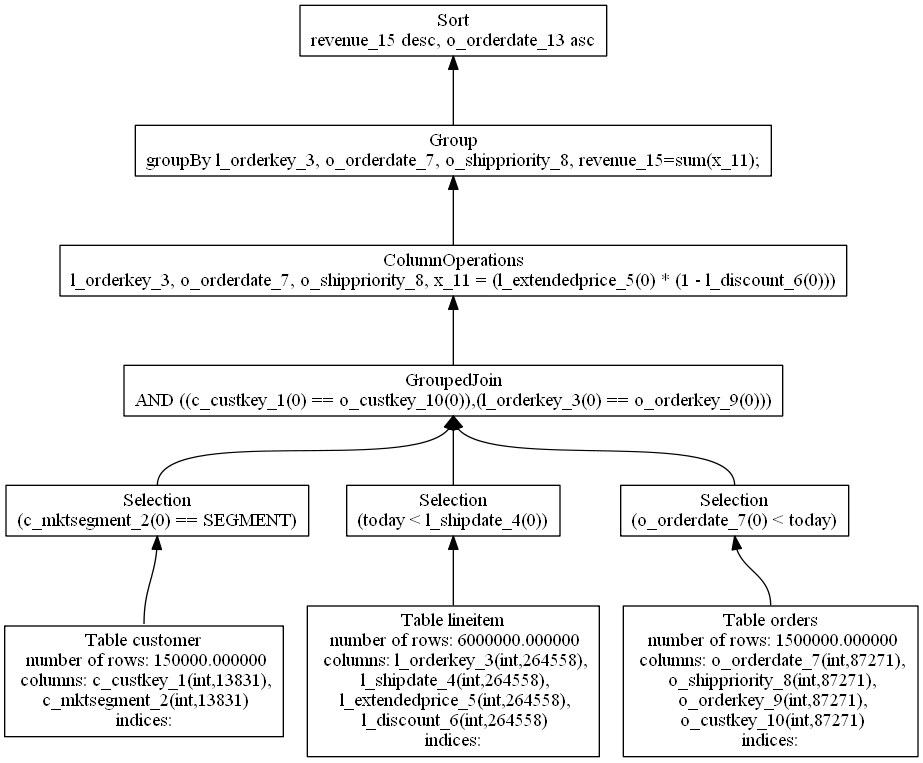
\includegraphics[width=1.0\textwidth]{algebratree2}

      \caption{Example of optimized algebra tree.}
          \label{fig:algebratree2}
\end{figure}
At this moment we have optimized tree, we can find selection chains in it. To resolve this problem we apply \texttt{SelectionFusingVisitor}. This visitor applies following rule to tree:
\begin{itemize}
\item $\sigma_{A}(\sigma_{B}(R))=\sigma_{A~and~B}(R)$
\end{itemize}

In figure~\ref{fig:algebratree2} we can see optimizes algebra tree. In comparison figure~\ref{fig:algebratree1}, this tree has grouped join with three input relations. Also big selection about joins has been split and moved down the tree. Some part of condition became join condition other were pushed down on of branches of grouped join. Then we can see that new tree has columns with assigned unique identifiers. Because we have this identifiers we don't need to know number of input for each column.

This input is optimized algebra tree. We can of course implement more optimizations to improve logical plan.

\section{Generating plan}

Final logical plan will be processed by \texttt{AlgebraCompiler}, which outputs $n$ best plans. $n$ is a constant in  \texttt{AlgebraCompiler} represented by variable \texttt{NUM\-BER\_\-OF\_\-PLANS}. 

This visitor visits node of algebra tree, the it calls itself on its children. We use generated plans in child nodes to create plans for current node. After that we store best plans in variable \texttt{result} relation size in variable \texttt{size} and output columns in variable \texttt{outputColumns}. 

In every node we generate all possible plans. Structure store in variable \texttt{result}, which is a heap. After inserting plan we remove slowest plan.

Physical plan is represented as polymorphic tree. 


In figure \ref{fig:physicalplan} we can see best generated physical plan for query presented on the beginning of this chapter. Every operator contains estimated size and time. Below that we can see output columns with their unique identifiers. Since read tables doesn't contain any indexes, we have to read all the tables and filter results. After that we can only use hash join, because sorting relations for merge join would be to expressive and nested loop join is not supported by runtime or compiler. From the result we compute new columns and use hash group algorithm. We didn't use sorted group, because input is not sorted and output has to be sorted by other than group column.

\begin{figure}[h!]
  \centering
    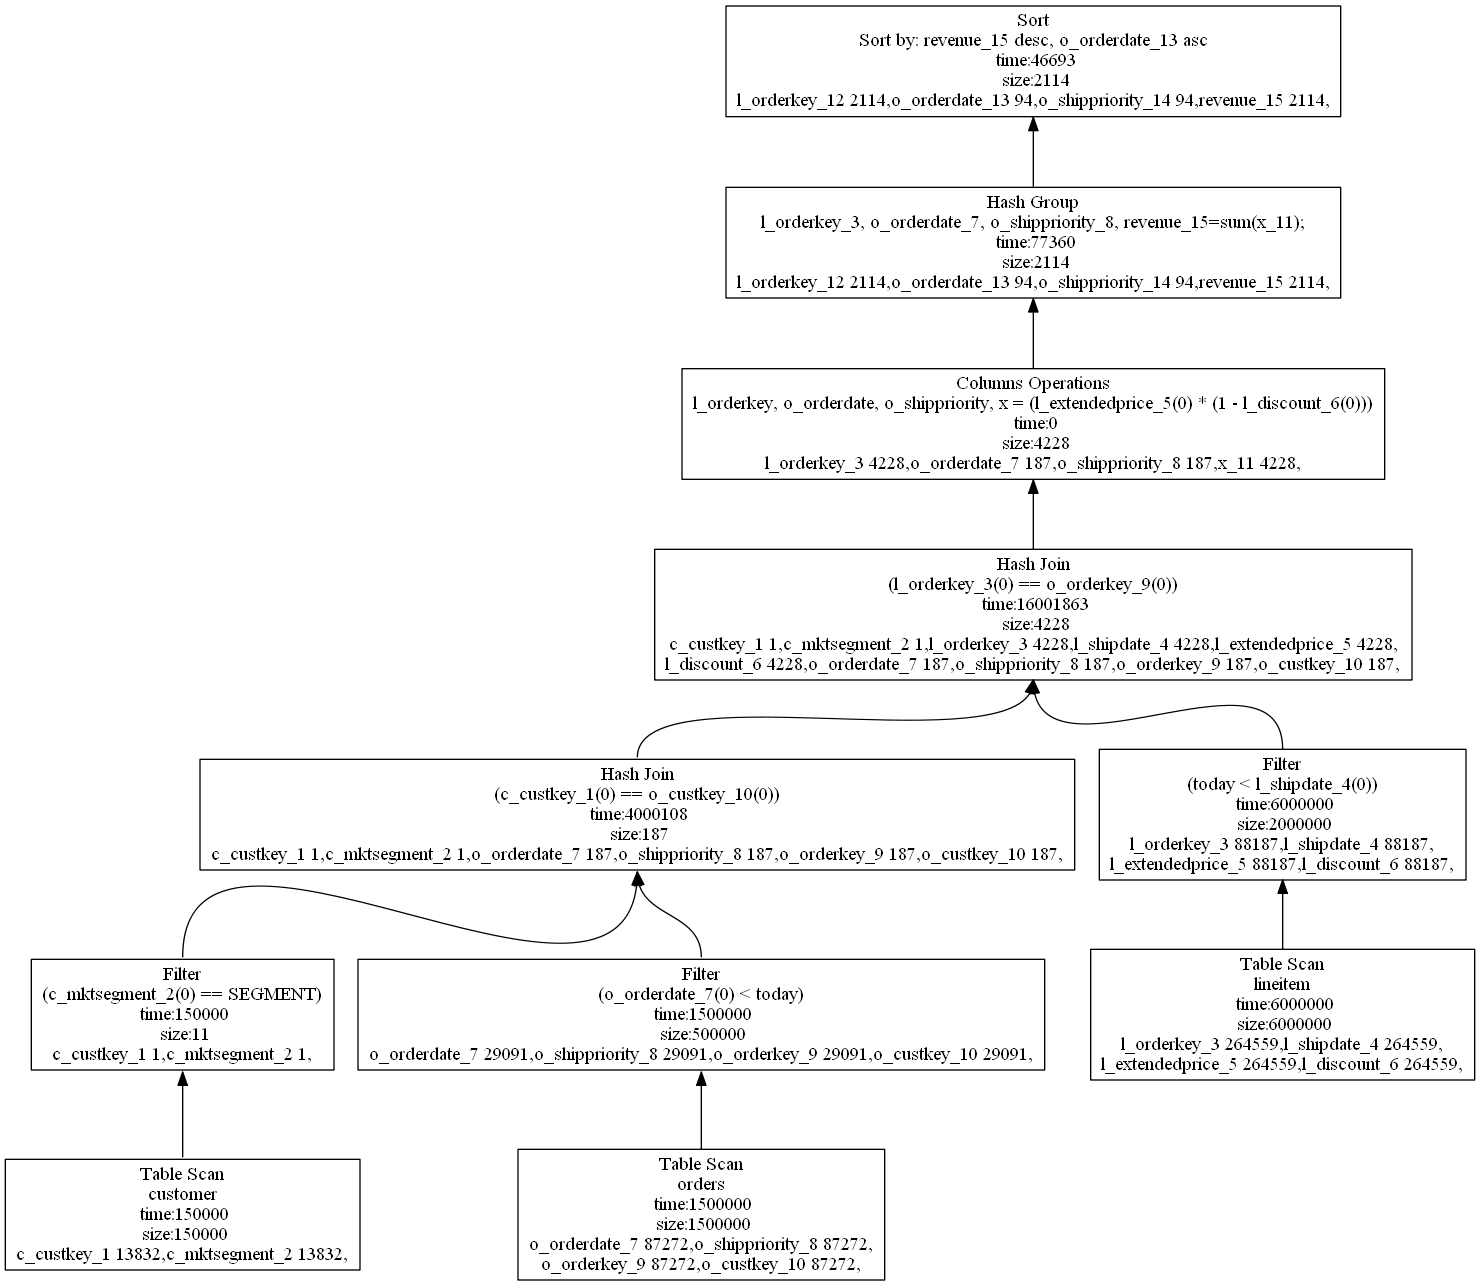
\includegraphics[width=1.0\textwidth]{physicalplan}

      \caption{Example of physical plan.}
          \label{fig:physicalplan}
\end{figure}

\section{Output}

In this section we describe text output generated by implemented compiler.

\subsection{Filters}
Example: 
\begin{lstlisting}
Filter(double,double,int)->(double,double,int)
f(condition="OP_LOWER(OP_double_CONSTANT(4.8),1)"); 
\end{lstlisting}

Input and output columns are the same and they are numbered from 0.
This operator takes input of two double streams and integer stream and it filters by condition $4.8<(column~number~1)$. We have also another version of this operator, which guaranteers that input and output are sorted the same way. To use it we write $FilterKeepingOrder$ instead of $Filter$ in operator declaration. 

\subsection{Group}
Example: 
\begin{lstlisting}
HashGroup(string,string,int)->(string,int,int)
g(groupBy="1",functions="count(),max(2)");
\end{lstlisting}
Input columns are numbered from 0. Output columns consists from grouped columns and computed aggregate functions in the same order as in parameters. 
This example groups by column number 1 and computes aggregate function $COUNT$ and $MAX$. $MAX$ has as parameter column number 2. 

We have also sorted version of this operators. It assumes that input is sorted by group columns. To use it we write $SortedGroup$ instead of $HashGroup$ in declaration.

\subsection{Column operations}
Example: 
\begin{lstlisting} 
ColumnsOperations(int,int,int,int,int)->(int,int,int,double)
c(out="0,3,4,OP_TIMES(2,OP_MINUS(OP_double_CONSTANT(1),2))"); 
\end{lstlisting}
Input columns are numbered from 0. Output is specified in parameter $out$. It if contains number operator, copies input to output, otherwise it computes new column. 
This example copies columns number $0,3,4$ to output and computes new column with expression: $2*(1-column~number~2)$.

\subsection{Cross join}
Example:
\begin{lstlisting} 
CrossJoin(string,int)(int,string)->(string,string)
c(left="0,1",right="2,3",out="0,3");
\end{lstlisting}
Numbering columns from first input is specified in $left$ parameter and numbering columns from second input is specified in $right$ parameter. Join outputs only columns given in $out$ argument. 

\subsection{Hash join}
Example:
\begin{lstlisting}
HashJoin(int,int)(int,int,int,int)->(int,int,int,int,int,int)
h(left="0,1",right="2,3,4,5",out="0,1,2,3,4,5",
leftPartOfCondition="0,1","rightPartOfCondition="5,2"); 
\end{lstlisting}
Numbering columns from first input is specified in $left$ parameter and numbering columns from second input is specified in $right$ parameter. Join outputs only columns given in $out$ argument. This operators works only with equal condition, which is given in parameters $leftPartOfCondition$ and $rightPartOfCondition$. This example computes join with condition:\\
 $(column~0=column~5)~and~(column~1=column~2)$.

\subsection{Merge equijoin}
Example:
\begin{lstlisting}
MergeEquiJoin(int)(int)->(int,int))
m(left="0",right="1",out="0,1",leftPartOfCondition="0:D",
rightPartOfCondition="1:D");
\end{lstlisting}
Numbering columns from first input is specified in $left$ parameter and numbering columns from second input is specified in $right$ parameter. Join outputs only columns given in $out$ argument. Condition is given in parameters $leftPartOfCondition$ and $rightPartOfCondition$ and they also contain information how are inputs sorted. This example computes join with condition $(0==1)$. First input is sorted by column number 0 descending and the second input is sorted by column 1 descending.

\subsection{Merge non equijoin}
Example:
\begin{lstlisting}
MergeNonEquiJoin(date,date)(date)->(date,date,date)
m(left="0,1",right="2",out="0,1,2",
leftInputSortedBy = "0:A,1:A",rightInputSortedBy = "2:A",
condition="OP_AND(OP_LOWER_OR_EQUAL(0,2)
,OP_LOWER_OR_EQUAL(2,1))");
\end{lstlisting}

This operator joins sorted relations. Numbering from left(first) and right(second) input is specified in parameters $left$ and $right$. Parameters $leftInputSortedBy$ and $rightInputSortedBy$ store information about how are input relations sorted. Join condition is in parameter $condition$. Operator in this example joins by condition $column~0 \leq column~2\leq column~1$. First input is sorted by column $0$ ascending and column $1$ ascending and second input is sorted by column $2$ ascending.

\subsection{Hash anti join}
Example:
\begin{lstlisting}
HashAntiJoin(int)(int)->(int)
h(left="0",right="1",out="0",leftPartOfCondition="0",
rightPartOfCondition="1"); 
\end{lstlisting}

Column number from first input is specified in $left$ parameter and columns numbers from second input is specified in $right$ parameter. Join outputs only columns given in $out$ argument. Parameter $out$ can only contains columns from first input. And specifies columns, which goes to output. Condition is given in parameters $leftPartOfCondition$ and $rightPartOfCondition$.This example computes antijoin with condition $(column~0==column~1)$.

\subsection{Merge anti join}
Example:
\begin{lstlisting}
$MergeAntiJoin(int)(int)->(int)
$m(left="0",right="1",out="0",leftPartOfCondition="0:D",
rightPartOfCondition="1:D");
\end{lstlisting}

Numbering columns from first input is specified in $left$ parameter and numbering columns from second input is specified in $right$ parameter. Join outputs only columns given in $out$ argument. Operator copies to output only rows from first input for which doesn't exist row in second input satisfying given condition.
Condition is given in parameters $leftPartOfCondition$ and $rightPartOfCondition$ and they also contain information how are inputs sorted. This example computes join with condition $(column~0==column~1)$. First input is sorted by column number 0 descending and the second input is sorted by 1 descending.

\subsection{Table scan}
Example:
\begin{lstlisting}
TableScan()->(int,int,int,int)
t(name="lineitem",
columns="l_orderkey,l_shipdate,l_extendedprice,l_discount");
\end{lstlisting}
This operator scans table specified in parameter $name$ and reads only columns given in parameter $columns$.

\subsection{Scan And Sort By Index}
Example:
\begin{lstlisting}
ScanAndSortByIndexScan()->(string,string,int)
s(name="people",index="index",
columns="user_name,country,parameter"); 
\end{lstlisting}
Operator reads whole table given in $name$ using $index$ and reads columns specified in attribute $columns$.

\subsection{Index Scan}

Example:
\begin{lstlisting}
IndexScan()->(int,int)
i(name="customer",index="index2",columns="c_custkey,c_mktsegment",
condition="OP_EQUALS(1,OP_string_CONSTANT(SEGMENT))");
\end{lstlisting}
Operator reads part of table given in $name$ using $index$ and reads columns specified in attribute $columns$. Operator reads only rows satisfying condition given in attribute $condtion$.



\subsection{Sort}
Example:
\begin{lstlisting}
SortOperator(int,int)->(int,int)
s(sortedBy="0",sortBy="1:D");
\end{lstlisting}
Input and output columns are the same and they are numbered from 0. Parameter $sortedBy$ specifies by which columns is table sorted and parameter $sortBy$ specifies by which columns should table be sorted. Example is already sorted by $colum~0$ and will be sorted by $column~1$ descending.


\subsection{Union}
Example:
\begin{lstlisting}
Union(int,string)(string,int)->(int,string)
u(left="0,1",right="1,0",out="0,1");
\end{lstlisting}
Numbering columns from the first input is given in the $left$ parameter, from second input is given in the $right$ parameter and from the output is given in the $out$ parameter.

